\chapter{ARN no codificantes y regulación postranscripcional}\label{ch:b3:rna-regulation}

En 1990 dos biólogos vegetales intentaron dar a unas petunias un morado
más intenso añadiéndoles copias del gen de la enzima del pigmento. Casi
la mitad de las plantas transgénicas salieron blancas, o moradas con
sectores blancos: el gen añadido había apagado también la copia propia de
la planta, además de a sí mismo. Ocho años después, dos genetistas de
gusanos que inyectaban ARN en \emph{Caenorhabditis elegans} descubrieron
que un ARN de doble hebra que correspondía a un gen muscular silenciaba
ese gen, en el gusano inyectado y en su descendencia, con mucha más
potencia que cualquiera de las dos hebras por separado. Los dos enigmas
tenían una sola respuesta: las células poseen una maquinaria que usa ARN
cortos para encontrar y silenciar ARN de secuencia correspondiente. Esa
maquinaria, y el mundo más amplio de la regulación que le ocurre a un ARN
mensajero después de transcrito --- cómo se corta y empalma, adónde se
envía, cuánto vive, si se traduce --- son el asunto de este capítulo. El
volumen de primer año trataba el gen como una unidad que se enciende o se
apaga en su promotor; aquí el objeto del control es el propio transcrito.

\section{El censo de ARN de una célula}

\begin{definition}[ARN no codificante]\label{def:b3:rna-regulation:ncrna}
\index{ARN no codificante}\index{microARN}\index{ARNip}\index{ARNpi}\index{ARN largo no codificante}\index{ARN nuclear pequeño}
Un \emph{ARN no codificante} (ncARN) es un transcrito que funciona como
ARN y no como molde de una proteína. Además de los ARN ribosómicos y de
transferencia de la traducción y de los \emph{ARN nucleares pequeños}
(snARN) del espliceosoma, una célula eucariota contiene: \emph{microARN}
(miARN), de \numrange{21}{23} nucleótidos, cortados de horquillas
presentes en los propios transcritos de la célula y que guían la
represión de mensajeros parcialmente complementarios; \emph{ARN pequeños
de interferencia} (ARNip), de la misma longitud, cortados de ARN largos
de doble hebra y que guían el corte de dianas perfectamente
complementarias; \emph{ARN que interaccionan con Piwi} (ARNpi), de
\numrange{26}{31} nucleótidos, activos en la línea germinal contra los
transposones; ARN nucleolares pequeños que guían la modificación del
ARNr; y \emph{ARN largos no codificantes} (lncARN), transcritos de más de
\qty{200}{nt} sin marco de lectura abierto de importancia, de los cuales
\emph{\omterm{def:b3:chromatin-epigenetics:x-inactivation}{Xist}}, del \cref{ch:b3:chromatin-epigenetics}, es el mejor
conocido. Los exones codificantes de proteína son alrededor del
\qty{1.5}{\%} del genoma humano; buena parte del resto se transcribe en
algún momento en alguna célula, pero cuánta de esa transcripción es
funcional es una cuestión abierta.
\end{definition}

\begin{remark}[Abundancia no es función]\label{rem:b3:rna-regulation:function}
Un transcrito puede detectarse porque la polimerasa tiene fugas, no
porque el ARN haga algo; la mayoría de los lncARN están presentes a menos
de una copia por célula, están poco conservados y son prescindibles
cuando se suprimen. La prueba de función es genética: un fenotipo cuando
se quita el ARN y no solo su ADN. \emph{\omterm{def:b3:chromatin-epigenetics:x-inactivation}{Xist}}, los miARN y los \omterm{def:b3:rna-regulation:ncrna}{ARNpi} la
superan con holgura; de las decenas de miles de lncARN anotados, unos
pocos centenares lo han hecho hasta ahora.
\end{remark}

\section{La interferencia por ARN y los microARN}

\begin{definition}[Interferencia por ARN]\label{def:b3:rna-regulation:rnai}
\index{interferencia por ARN}\index{Dicer}\index{Argonauta}\index{RISC}
La \emph{interferencia por ARN} (ARNi) es el silenciamiento específico de
secuencia de un gen por un ARN pequeño derivado de un ARN de doble hebra.
La enzima \emph{Dicer}, una ARNasa III, corta el ARN largo de doble hebra
en dúplex de \numrange{21}{23} nucleótidos con extremos 3$'$ salientes de
dos nucleótidos; una hebra de cada dúplex, la guía, se carga en una
proteína \emph{Argonauta} para formar el \emph{complejo silenciador
inducido por ARN} (RISC). La guía se aparea con un ARN diana
complementario, y el dominio endonucleasa de Argonauta corta la diana
frente a los nucleótidos 10 y 11 de la guía; el ARN cortado se degrada
después y el RISC queda libre para buscar otro. En plantas, gusanos y
hongos una ARN-polimerasa dependiente de ARN copia la diana en nuevo ARN
de doble hebra, con lo que la señal se amplifica y se propaga; los
mamíferos carecen de este paso.
\end{definition}

\begin{proof}[Evidencia]
Napoli, Lemieux y Jorgensen (1990) introdujeron en la petunia un gen
adicional de la chalcona-sintasa para intensificar el color de la flor;
el \qty{42}{\%} de los transformantes salieron blancos o variegados, con
el transgén y el gen endógeno silenciados los dos --- la
``cosupresión''. Guo y Kemphues (1995) encontraron que un ARN
antisentido contra un gen de \emph{C.~elegans} lo silenciaba, pero
también lo hacía el control con sentido. Fire, Mello y colaboradores
(1998) resolvieron la paradoja: sus preparaciones de hebras sencillas
estaban contaminadas con hebras dobles, y el ARN de doble hebra
purificado de \emph{unc-22} inyectado en un gusano dio el fenotipo de
espasmos de \emph{unc-22} a concentraciones de unas pocas moléculas por
célula, mientras que el ARN con sentido o antisentido puro no dio casi
nada; el silenciamiento pasaba a tejidos lejanos del punto de inyección y
a la descendencia. Hamilton y Baulcombe (1999) detectaron los ARN de
\qty{25}{nt} en plantas silenciadas, y Zamore y colaboradores (2000)
mostraron en un extracto de mosca que el ARN de doble hebra se corta en
ellos y que la diana se corta a intervalos de \qty{21}{nt}.
\end{proof}

\begin{omfigure}
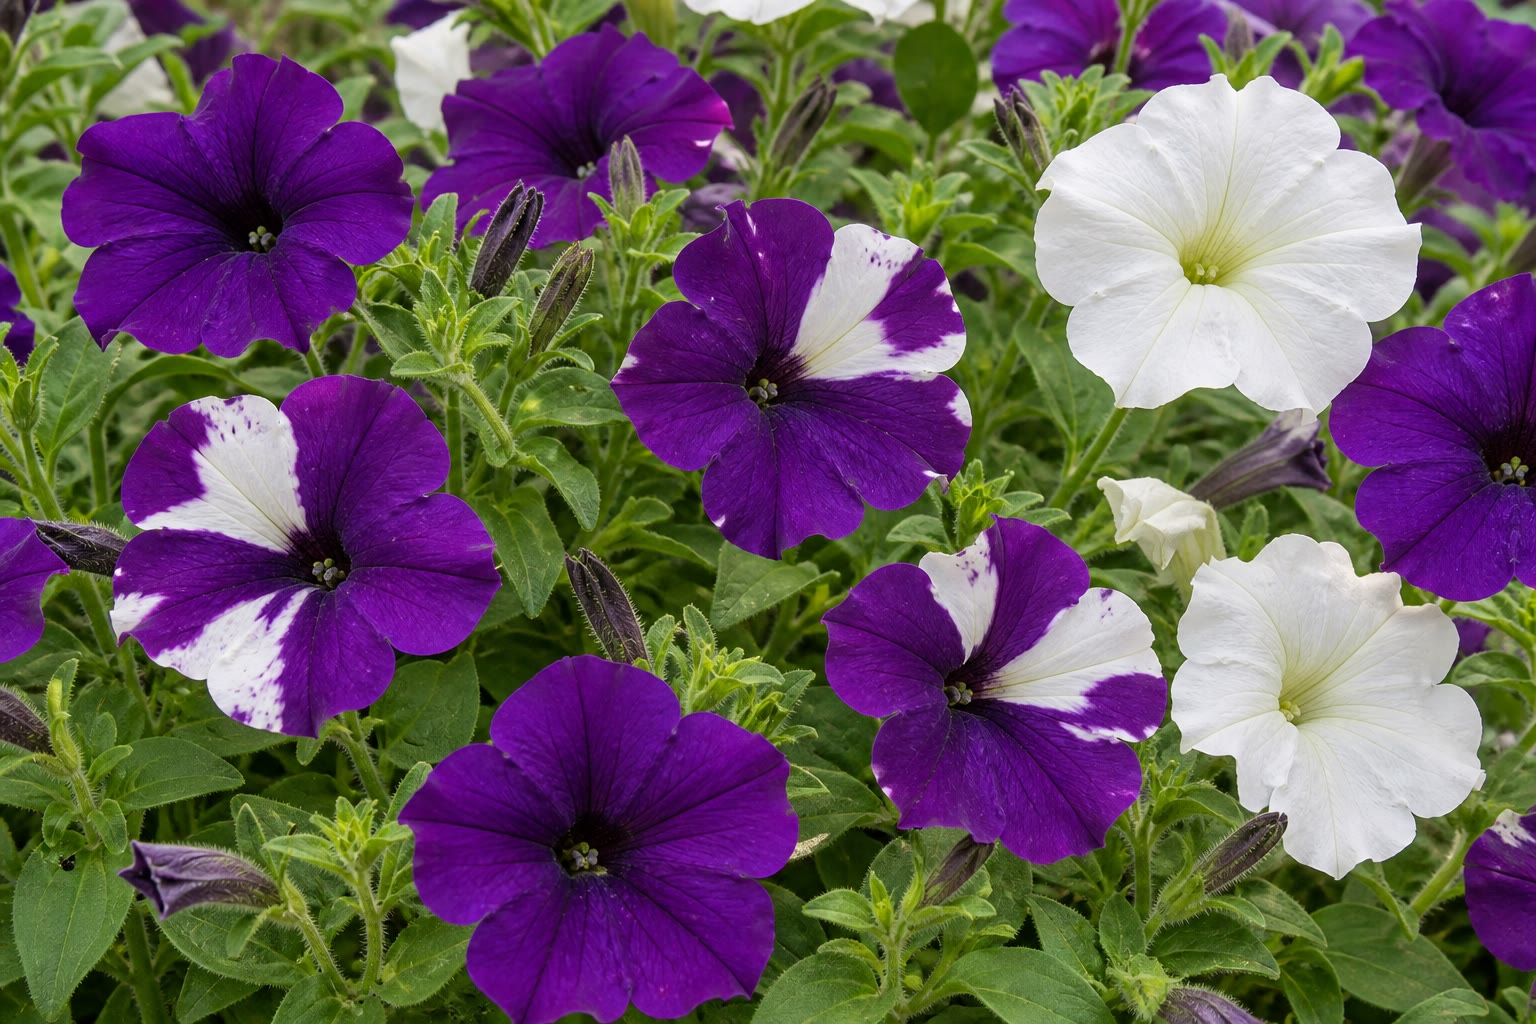
\includegraphics[width=0.46\linewidth]{images/book5/ai/b5-02-petunia-cosuppression.jpg}\hspace{0.04\linewidth}
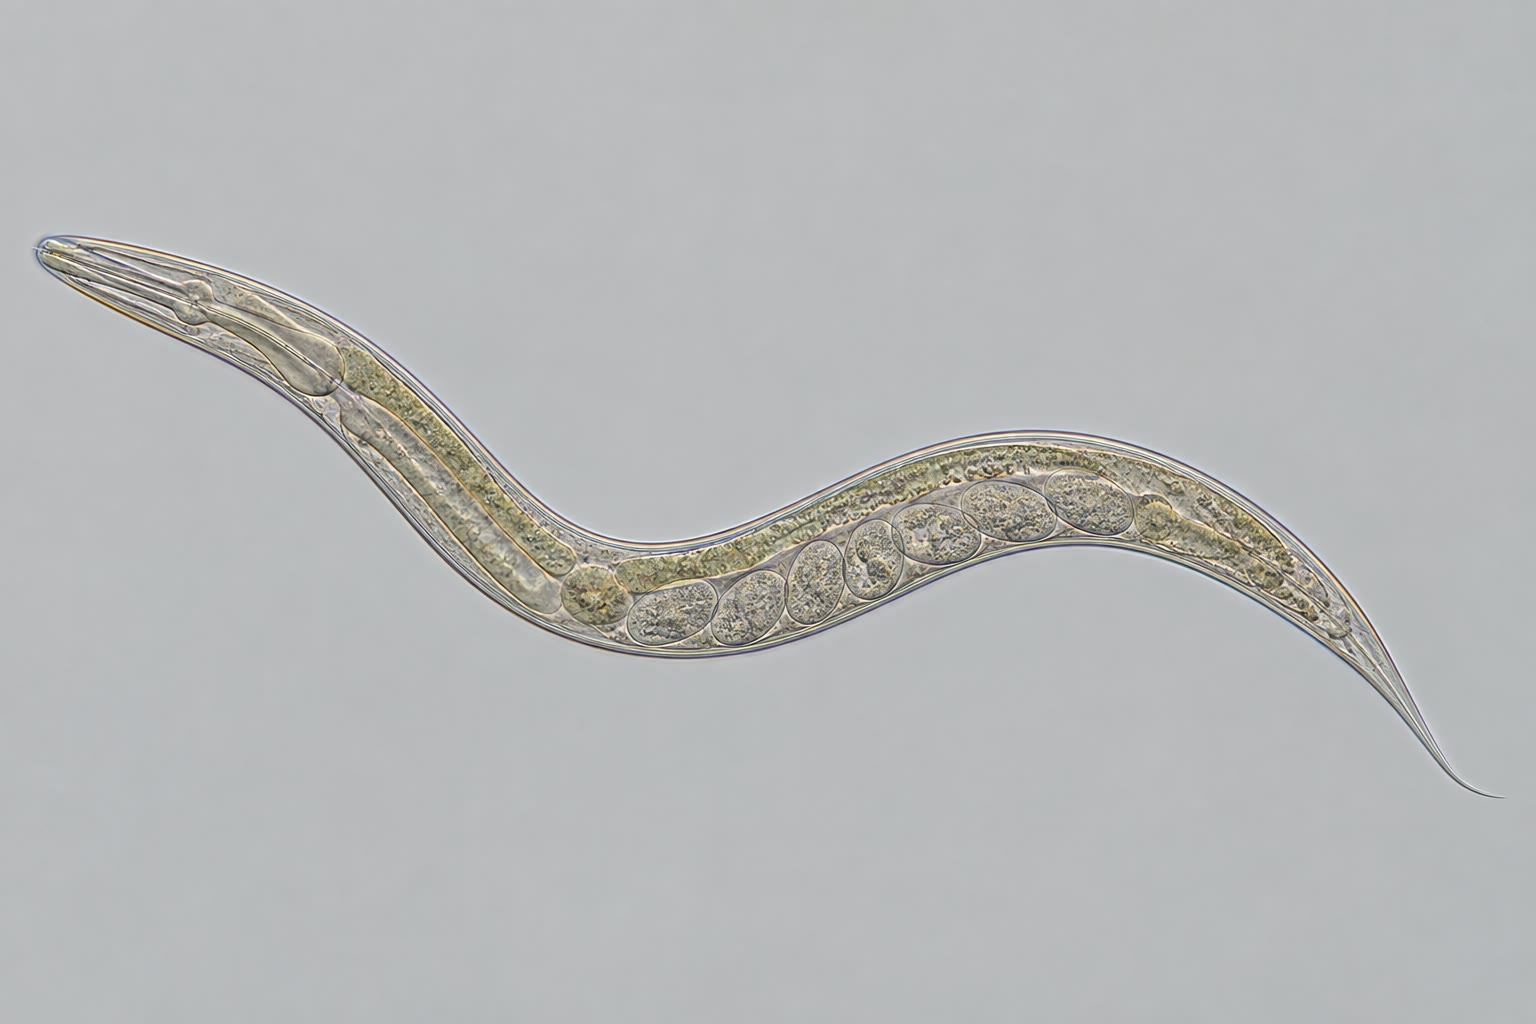
\includegraphics[width=0.46\linewidth]{images/book5/ai/b5-02-c-elegans.jpg}

{\small Izquierda: petunias que llevan un gen adicional del pigmento, con
los sectores blancos de la cosupresión. Derecha: el nematodo
\emph{Caenorhabditis elegans}, de alrededor de un milímetro y
transparente, en el que un ARN de doble hebra inyectado silenció el gen
correspondiente en todo el animal y en su descendencia.}
\end{omfigure}

\begin{definition}[MicroARN]\label{def:b3:rna-regulation:mirna}
\index{microARN!biogénesis}\index{Drosha}\index{secuencia semilla}
Un \emph{\omterm{def:b3:rna-regulation:ncrna}{microARN}} está codificado en el genoma --- en un gen propio o en
un intrón de un gen codificante de proteína --- y lo transcribe la
ARN-polimerasa II como un transcrito primario largo (pri-miARN) que
contiene una horquilla de unos \qty{70}{nt}. En el núcleo la ARNasa III
\emph{Drosha}, con su pareja DGCR8, recorta la horquilla (el pre-miARN);
la exportina-5 la lleva al citoplasma, donde \omterm{def:b3:rna-regulation:rnai}{Dicer} retira el bucle y deja
un dúplex de \qty{22}{nt}. Una hebra se carga en \omterm{def:b3:rna-regulation:rnai}{Argonauta}. El miARN
maduro reconoce sus dianas sobre todo por su \emph{semilla}, los
nucleótidos 2 a 8, que se aparea con sitios situados casi siempre en la
región 3$'$ no traducida de un mensajero; el resto del miARN se aparea de
forma imperfecta, de modo que la diana no se corta sino que se reprime:
el \omterm{def:b3:rna-regulation:rnai}{RISC} recluta proteínas que acortan la cola de poli(A), quitan la
caperuza e inhiben la traducción, y el mensajero se degrada más deprisa.
Como una semilla tiene solo siete nucleótidos, un miARN tiene centenares
de dianas, y más de la mitad de los genes humanos codificantes de
proteína llevan sitios conservados para al menos uno de los varios
centenares de miARN humanos identificados con seguridad.
\end{definition}

\begin{proof}[Evidencia]
\emph{lin-4}, un gen que el gusano necesita para pasar de su primer
estadio larvario al segundo, resultó, según Lee, Feinbaum y Ambros
(1993), codificar no una proteína sino un ARN de \qty{22}{nt},
complementario de siete sitios de la región 3$'$ no traducida del
mensajero de \emph{lin-14}, el gen que se sabía que reprimía. Cuando la
larva entra en el segundo estadio, la proteína LIN-14 desaparece mientras
su ARNm permanece: la represión es postranscripcional. Reinhart y
colaboradores (2000) hallaron un segundo ARN de esta clase,
\emph{let-7}, que controla las transiciones larvarias posteriores;
Pasquinelli (2000) encontró \emph{let-7} en moscas y en humanos, con la
misma secuencia, lo que convirtió una curiosidad de gusano en un
mecanismo general.
\end{proof}

\begin{omfigure}
\begin{tikzpicture}[every node/.style={font=\scriptsize}, >=stealth]
  % nucleus box
  \draw[rounded corners=8pt, thick, gray!60, fill=gray!6] (-0.4,-1.1) rectangle (5.2,2.7);
  \node[gray, anchor=south west] at (-0.3,-1.05) {núcleo};
  % gene and pri-miRNA
  \draw[very thick, omDef] (0,2.0) -- (2.4,2.0); \node[above] at (1.2,2.05) {gen de miARN, Pol II};
  \draw[->, thick] (1.2,1.85) -- (1.2,1.35);
  % hairpin
  \draw[thick, omThm!70!black] (0.2,1.0) -- (0.9,1.0) .. controls (1.0,1.0) and (1.05,0.9) .. (1.1,0.5) .. controls (1.15,0.1) and (1.25,0.1) .. (1.3,0.5) .. controls (1.35,0.9) and (1.4,1.0) .. (1.5,1.0) -- (2.2,1.0);
  \draw[thick, omThm!70!black] (1.1,0.5) -- (1.3,0.5);
  \node[below] at (1.2,0.0) {horquilla pri-miARN};
  % Drosha
  \draw[thick, fill=omExo!35] (2.9,0.7) ellipse (0.55 and 0.28); \node at (2.9,0.7) {Drosha};
  \draw[->, thick] (2.3,0.85) -- (2.4,0.75);
  \draw[->, thick] (3.5,0.7) -- (4.2,0.7) node[midway, above] {corte};
  % pre-miRNA
  \draw[thick, omThm!70!black] (4.3,0.9) .. controls (4.5,0.9) and (4.55,0.4) .. (4.6,0.1) .. controls (4.65,-0.2) and (4.75,-0.2) .. (4.8,0.1) .. controls (4.85,0.4) and (4.9,0.9) .. (5.1,0.9);
  \node[below, align=center] at (4.7,-0.25) {pre-miARN\\\qty{70}{nt}};
  % export
  \draw[->, thick] (5.35,0.4) -- (6.3,0.4) node[midway, above, xshift=0.2cm] {exportina-5};
  % cytoplasm
  \node[gray, anchor=north west] at (5.5,2.65) {citoplasma};
  \draw[thick, fill=omExo!35] (6.9,0.4) ellipse (0.5 and 0.28); \node at (6.9,0.4) {Dicer};
  \draw[->, thick] (7.45,0.4) -- (8.1,0.4);
  \draw[thick, omThm!70!black] (8.2,0.55) -- (9.6,0.55); \draw[thick, omThm!70!black] (8.35,0.25) -- (9.75,0.25);
  \node[below, align=center] at (8.95,0.15) {dúplex de \qty{22}{nt}};
  \draw[->, thick] (8.95,-0.4) -- (8.95,-0.9) node[midway, right] {se carga una hebra};
  % RISC on mRNA
  \draw[thick, fill=omProp!35] (8.95,-1.45) ellipse (0.85 and 0.35); \node at (8.95,-1.45) {Argonauta};
  \draw[thick, omThm!70!black] (8.3,-1.85) -- (9.6,-1.85);
  \draw[very thick, omDef] (5.6,-2.15) -- (11.4,-2.15);
  \node[below] at (6.4,-2.2) {ARNm: región codificante}; \node[below] at (10.3,-2.2) {3$'$ UTR, sitio diana};
  \draw[omDef, thick] (11.4,-2.15) -- (11.8,-2.15) node[right] {AAAA};
  \draw[->, thick, omThm] (9.9,-1.5) -- (10.9,-1.5) node[right, align=left] {desadenilación,\\degradación, menos\\traducción};
  \node[below, align=center] at (8.95,-2.7) {la semilla (nt 2--8) se\\aparea con el sitio};
\end{tikzpicture}

{\small Biogénesis de un \omterm{def:b3:rna-regulation:ncrna}{microARN}. \omterm{def:b3:rna-regulation:mirna}{Drosha} recorta la horquilla del
transcrito primario en el núcleo, se exporta, \omterm{def:b3:rna-regulation:rnai}{Dicer} la recorta hasta un
dúplex de \qty{22}{nt} y una hebra se carga en \omterm{def:b3:rna-regulation:rnai}{Argonauta}. La semilla se
aparea con un sitio de la región 3$'$ no traducida de un mensajero, y el
mensajero se desadenila, se degrada y se traduce menos.}
\end{omfigure}

\begin{theorem}[Lo que un microARN hace al nivel y a la velocidad de un mensajero]\label{thm:b3:rna-regulation:mirna-kinetics}
\index{semivida del ARNm}\index{tiempo de respuesta}
Un mensajero se sintetiza a velocidad constante $k$ y se degrada con
velocidad de primer orden $\gamma$; un \omterm{def:b3:rna-regulation:ncrna}{microARN} presente a nivel $R$
añade un término de degradación $\gamma' R\, m$. El nivel de ARNm $m(t)$
obedece entonces
\[
\frac{\mathrm{d}m}{\mathrm{d}t} = k - (\gamma + \gamma' R)\, m,
\qquad
m^{*} = \frac{k}{\gamma + \gamma' R},
\qquad
m(t) = m^{*} + (m_{0} - m^{*})\,e^{-(\gamma + \gamma' R)t}.
\]
El \omterm{def:b3:rna-regulation:ncrna}{microARN} rebaja el estado estacionario por el factor $1 + \gamma' R/
\gamma$ y acorta por ese mismo factor la constante de tiempo de todo
cambio de $m$, de $1/\gamma$ a $1/(\gamma + \gamma' R)$. Un gen regulado
por \omterm{def:b3:rna-regulation:ncrna}{microARN} es por tanto a la vez más silencioso y más rápido: alcanza
antes un nuevo estado estacionario después de que cambie su promotor, y
las fluctuaciones de su transcripción quedan amortiguadas.
\end{theorem}
\begin{proof}
La ecuación es lineal de coeficientes constantes; su punto fijo es
$m^{*}$, donde se anula el miembro derecho, y escribiendo $u = m - m^{*}$
resulta $\mathrm{d}u/\mathrm{d}t = -(\gamma + \gamma' R)\,u$, de donde la
exponencial. El semitiempo de la aproximación es $\ln 2/(\gamma + \gamma'
R)$, y $\gamma = \ln 2 / t_{1/2}$, donde $t_{1/2}$ es la semivida natural
del mensajero.
\end{proof}

\begin{example}[Una represión de cuatro veces]\label{ex:b3:rna-regulation:fourfold}
Un mensajero con una semivida natural de \qty{30}{min} ($\gamma =
\qty{0.023}{min^{-1}}$), transcrito a $k = 2$ moléculas por minuto, se
sitúa en $m^{*} = 2/0.023 \approx 87$ copias por célula y tarda
\qty{30}{min} en recorrer la mitad del camino hasta un nivel nuevo
después de que cambie su promotor. Un \omterm{def:b3:rna-regulation:ncrna}{microARN} que triplique su velocidad
de degradación ($\gamma' R = 3\gamma$) lo lleva a $22$ copias y reduce el
semitiempo a \qty{7.5}{min}. Los mismos números, leídos al revés,
explican por qué las supresiones de miARN suelen tener fenotipos leves:
un cambio de cuatro veces en un mensajero que a su vez está amortiguado
aguas abajo puede dejar al organismo casi normal, y el efecto se
manifiesta bajo estrés o en la temporización.
\end{example}

\begin{omfigure}
\begin{tikzpicture}
\begin{axis}[
  width=0.7\linewidth, height=5.6cm,
  axis x line=bottom, axis y line=left,
  xmin=0, xmax=120, ymin=0, ymax=100,
  xlabel={tiempo tras el encendido del promotor (min)}, ylabel={ARNm por célula},
  xlabel style={font=\small, at={(axis description cs:0.5,-0.12)}, anchor=north},
  ylabel style={font=\small},
  tick label style={font=\small}, xtick={0,30,60,90,120}, ytick={0,22,50,87},
  clip=false,
]
\addplot[very thick, omDef, domain=0:120, samples=80] {87*(1-exp(-0.0231*x))};
\addplot[very thick, omThm, domain=0:120, samples=80] {21.7*(1-exp(-0.0924*x))};
\addplot[dashed, gray, domain=0:120, samples=2] {87};
\addplot[dashed, gray, domain=0:120, samples=2] {21.7};
\node[font=\scriptsize, omDef, anchor=south west] at (axis cs:5,90) {sin microARN: $m^{*} = 87$, semitiempo \qty{30}{min}};
\node[font=\scriptsize, omThm, anchor=south west] at (axis cs:40,24) {con microARN, $\gamma' R = 3\gamma$: $m^{*} = 22$, semitiempo \qty{7.5}{min}};
\end{axis}
\end{tikzpicture}

{\small Ascenso de un mensajero tras encenderse su promotor, con los
números del \cref{ex:b3:rna-regulation:fourfold}. El \omterm{def:b3:rna-regulation:ncrna}{microARN} baja la
meseta cuatro veces y la alcanza cuatro veces antes.}
\end{omfigure}

\begin{method}[Silenciar un gen con ARNi]\label{met:b3:rna-regulation:knockdown}
\index{silenciamiento parcial}\index{ARNhc}
Para silenciar un gen sin tocar su ADN: (1) elíjase una secuencia de
\qty{21}{nt} propia de su mensajero, evitando coincidencias de semilla
con otros genes; (2) entréguese como un dúplex de \omterm{def:b3:rna-regulation:ncrna}{ARNip} sintético
(transitorio, unos pocos días) o como un ARN en horquilla corta (ARNhc)
expresado desde un vector, que \omterm{def:b3:rna-regulation:rnai}{Dicer} procesa de continuo; en los gusanos,
aliméntense los animales con bacterias que expresan el ARN de doble
hebra; (3) mídase el mensajero por PCR cuantitativa y la proteína por
inmunotransferencia, esperando una pérdida del \qtyrange{70}{95}{\%} y no
la ausencia completa de una supresión génica; (4) contrólense los efectos
fuera de diana con un segundo \omterm{def:b3:rna-regulation:ncrna}{ARNip} que no se solape y con un rescate
mediante una versión del gen resistente al ARNi. Un \omterm{met:b3:rna-regulation:knockdown}{silenciamiento
parcial} es una pérdida de función parcial y reversible; las terapias
génicas ya aprobadas sobre este principio entregan \omterm{def:b3:rna-regulation:ncrna}{ARNip} contra
mensajeros hepáticos (transtiretina, PCSK9) acoplados a un azúcar que el
hepatocito capta.
\end{method}

\section{ARN pequeños que vigilan el genoma}

\begin{definition}[Los ARNpi y el silenciamiento de transposones]\label{def:b3:rna-regulation:pirna}
\index{ARNpi!ping-pong}\index{silenciamiento de transposones}\index{disgenesia híbrida}
Los \emph{\omterm{def:b3:rna-regulation:ncrna}{ARNpi}} son ARN de \numrange{26}{31} nucleótidos, fabricados sin
\omterm{def:b3:rna-regulation:rnai}{Dicer} a partir de transcritos largos de hebra sencilla de los
\emph{agrupamientos de \omterm{def:b3:rna-regulation:ncrna}{ARNpi}} del genoma --- cementerios de copias
defectuosas de transposones --- y cargados en la subfamilia PIWI de las
proteínas \omterm{def:b3:rna-regulation:rnai}{Argonauta} en la línea germinal. Un \omterm{def:b3:rna-regulation:ncrna}{ARNpi} antisentido de un
transposón guía el corte de los transcritos del transposón; el fragmento
cortado se convierte en un nuevo \omterm{def:b3:rna-regulation:ncrna}{ARNpi} con sentido, que a su vez corta
transcritos del agrupamiento para fabricar más \omterm{def:b3:rna-regulation:ncrna}{ARNpi} antisentido --- el
ciclo \emph{ping-pong}, una amplificación dirigida contra el transposón
que esté activo en ese momento. Las proteínas PIWI nucleares dirigen
además la metilación de H3K9 y la \omterm{def:b3:chromatin-epigenetics:methylation}{metilación del ADN} hacia las copias
genómicas del transposón, y conectan así el ARN con las marcas de
\omterm{def:b3:chromatin-epigenetics:nucleosome}{cromatina} del \cref{ch:b3:chromatin-epigenetics}. La madre deposita sus
\omterm{def:b3:rna-regulation:ncrna}{ARNpi} en el óvulo; una hembra cuyo linaje nunca se ha encontrado con un
transposón no tiene \omterm{def:b3:rna-regulation:ncrna}{ARNpi} contra él, y su descendencia con un macho que
lo lleva es estéril --- la \emph{disgenesia híbrida}, vista por primera
vez en cruces de \emph{Drosophila} entre cepas de laboratorio y
silvestres.
\end{definition}

\begin{proposition}[Silenciamiento de la cromatina dirigido por ARN]\label{prop:b3:rna-regulation:rddm}
\index{metilación del ADN dirigida por ARN}
En las plantas, una vía dedicada --- la ARN-polimerasa IV transcribe un
locus, una ARN-polimerasa dependiente de ARN lo hace bicatenario, un
\omterm{def:b3:rna-regulation:rnai}{Dicer} corta \omterm{def:b3:rna-regulation:ncrna}{ARNip} de \qty{24}{nt}, \omterm{def:b3:rna-regulation:rnai}{Argonauta}~4 los lleva de vuelta a los
transcritos nacientes de la polimerasa V en ese mismo locus y recluta a
la metiltransferasa DRM2 --- metila el ADN de los transposones y de las
secuencias repetidas; es el mecanismo de la paramutación. En la levadura
de fisión, los \omterm{def:b3:rna-regulation:ncrna}{ARNip} de las repeticiones centroméricas reclutan a la
metiltransferasa de H3K9 y construyen la \omterm{def:b3:chromatin-epigenetics:nucleosome}{heterocromatina} que el
centrómero necesita. En ambos casos un ARN encuentra un lugar del genoma
por complementariedad y allí se escribe una marca de \omterm{def:b3:chromatin-epigenetics:nucleosome}{cromatina}:
específica de secuencia, autorreforzante y heredable a través de las
divisiones.
\end{proposition}

\section{La vida de un mensajero}

\begin{definition}[Corte y empalme regulados]\label{def:b3:rna-regulation:splicing}
\index{corte y empalme alternativo!regulación}\index{proteína SR}\index{hnRNP}\index{salto de exón}
El corte y empalme alternativo produce mensajeros distintos a partir de
un solo gen mediante el \emph{salto de exón}, la elección entre exones
mutuamente excluyentes, la retención de un intrón o el uso de sitios de
corte 5$'$ o 3$'$ alternativos. Lo regulan proteínas de unión al ARN que
reconocen elementos de secuencia de los exones y los intrones próximos a
un sitio de corte: las \emph{proteínas SR} unidas a potenciadores
exónicos reclutan al espliceosoma y favorecen la inclusión del exón, las
proteínas \emph{hnRNP} unidas a silenciadores la bloquean, y el resultado
en una célula dada lo fijan las cantidades relativas de los dos tipos.
Más del \qty{90}{\%} de los genes humanos con varios exones sufren corte
y empalme alternativo; el gen \emph{Dscam} de \emph{Drosophila}, con
cuatro bloques de exones mutuamente excluyentes (12, 48, 33 y 2
alternativas), puede producir \num{38016} proteínas distintas, y cada
neurona expresa un conjunto diferente que permite a sus ramas
reconocerse y evitarse entre sí.
\end{definition}

\begin{proof}[Evidencia]
El sexo de una mosca del vinagre lo decide una cascada de corte y
empalme. En las hembras el gen \emph{Sex-lethal} (\emph{Sxl}) produce una
proteína funcional; SXL es una proteína de unión al ARN que bloquea un
sitio de corte en su propio transcrito (de modo que se salta un exón con
codón de parada y la proteína se sigue produciendo) y en el transcrito de
\emph{transformer}, lo que fuerza el corte femenino; TRA, junto con
TRA-2, se une entonces a un potenciador exónico del transcrito de
\emph{doublesex} y dirige la forma femenina del factor de transcripción
DSX. En los machos, sin SXL, todos estos transcritos siguen el corte por
defecto, \emph{transformer} contiene un codón de parada y DSX sale en su
forma masculina. Todo rasgo sexualmente dimórfico de la mosca se sigue de
qué DSX se fabrique; una hembra con \emph{tra} mutado se desarrolla como
macho.
\end{proof}

\begin{definition}[Estabilidad y localización del ARNm]\label{def:b3:rna-regulation:stability}
\index{elemento rico en AU}\index{localización del ARNm}\index{elemento de respuesta al hierro}
La \emph{semivida} de un mensajero va de minutos a días y la fijan
elementos de su región 3$'$ no traducida. Los \emph{elementos ricos en
AU} (repeticiones AUUUA) de los mensajeros de citocinas, factores de
crecimiento y protooncogenes los unen proteínas que reclutan
desadenilasas y dan semividas de \qtyrange{10}{30}{min}, de modo que un
estallido de transcripción produce un estallido de proteína y nada más;
las mutaciones que los eliminan causan sobreexpresión y, en algunos
protooncogenes, cáncer. Los \emph{elementos de localización}, a menudo
estructurados, los unen adaptadores que enlazan el mensajero con un
motor: los mensajeros de \emph{bicoid} y de \emph{oskar} los llevan la
dineína y la cinesina sobre microtúbulos a los dos polos del huevo de la
mosca, el mensajero de la $\beta$-actina al borde delantero de un
fibroblasto y los mensajeros de las proteínas sinápticas a las dendritas,
donde se traducen a demanda. El \emph{elemento de respuesta al hierro}
(IRE), un tallo--bucle que unen las proteínas reguladoras del hierro IRP1
e IRP2 cuando el hierro escasea, hace dos trabajos opuestos desde dos
posiciones: en la región 5$'$ no traducida del mensajero de la ferritina,
la IRP unida bloquea al ribosoma; en la región 3$'$ no traducida del
mensajero del receptor de transferrina, la IRP unida protege al
transcrito de una nucleasa.
\end{definition}

\begin{example}[El hierro, leído por una horquilla]\label{ex:b3:rna-regulation:iron}
Cuando el hierro es escaso, la IRP une los dos mensajeros: la ferritina,
la proteína de almacenamiento, no se traduce, y el receptor de
transferrina, que importa hierro, se estabiliza y abunda --- la célula
almacena menos e importa más. Cuando el hierro es abundante, convierte a
IRP1 en una aconitasa (adquiere un agregado de hierro y azufre y pierde
su afinidad por el ARN) y desencadena la degradación de IRP2: la
ferritina se traduce, el mensajero del receptor decae en minutos, y la
célula almacena más e importa menos. No hace falta ningún cambio de
transcripción. Una mutación puntual del IRE de la ferritina que impide la
unión de la IRP causa una síntesis constitutiva de ferritina y el
síndrome hereditario de hiperferritinemia con cataratas.
\end{example}

\begin{omfigure}
\begin{tikzpicture}[every node/.style={font=\scriptsize}, >=stealth]
  \foreach \yy/\state in {2.2/hierro escaso, -0.9/hierro abundante} {
    \node[left, font=\small\bfseries] at (-0.2,\yy+0.35) {\state};
    % ferritin mRNA
    \draw[very thick, omDef] (0.3,\yy+0.6) -- (4.6,\yy+0.6); \node[below] at (3.3,\yy+0.4) {ARNm de ferritina};
    \draw[thick, omThm!70!black] (0.9,\yy+0.6) .. controls (0.9,\yy+1.15) and (1.3,\yy+1.15) .. (1.3,\yy+0.6); \node[below] at (1.1,\yy+0.55) {IRE};
    \draw[fill=omDef!20, thick] (2.2,\yy+0.42) rectangle (4.4,\yy+0.78);
    % TfR mRNA
    \draw[very thick, omDef] (6.2,\yy+0.6) -- (10.6,\yy+0.6); \node[below, font=\tiny] at (7.1,\yy+0.4) {ARNm del receptor de transferrina};
    \draw[fill=omDef!20, thick] (6.4,\yy+0.42) rectangle (8.6,\yy+0.78);
    \foreach \x in {9.0,9.5,10.0} \draw[thick, omThm!70!black] (\x,\yy+0.6) .. controls (\x,\yy+1.1) and (\x+0.35,\yy+1.1) .. (\x+0.35,\yy+0.6);
    \node[below, font=\tiny] at (9.9,\yy+0.55) {IRE (3$'$ UTR)};
  }
  % low iron: IRP bound
  \draw[thick, fill=omProp!40] (1.1,3.35) ellipse (0.4 and 0.24); \node at (1.1,3.35) {IRP};
  \node[right, omThm] at (1.55,3.35) {ribosoma bloqueado: no hay ferritina};
  \foreach \x in {9.18,9.68,10.18} { \draw[thick, fill=omProp!40] (\x,3.35) ellipse (0.28 and 0.2); }
  \node[above, omMeth!70!black] at (9.7,3.75) {protegido de la nucleasa: receptor abundante};
  \node[below, omMeth!70!black] at (1.1,1.75) {almacena menos};
  \node[below, omMeth!70!black] at (7.4,1.75) {importa más};
  % high iron: IRP off
  \node[right, omMeth!70!black] at (1.55,0.25) {se traduce: se fabrica ferritina};
  \node[right, omThm, align=left] at (10.7,-0.3) {nucleasa:\\el ARNm decae};
  \node[below, omThm] at (1.1,-1.35) {almacena más};
  \node[below, omThm] at (7.4,-1.35) {importa menos};
\end{tikzpicture}

{\small El \omterm{def:b3:rna-regulation:stability}{elemento de respuesta al hierro}. Con hierro escaso, la
proteína reguladora del hierro une las horquillas IRE: en el extremo 5$'$
del mensajero de la ferritina bloquea la traducción, y en el extremo 3$'$
del mensajero del receptor de transferrina bloquea a una nucleasa. Con
hierro abundante la proteína suelta ambos: se fabrica ferritina y el
mensajero del receptor decae.}
\end{omfigure}

\begin{proposition}[Control traduccional]\label{prop:b3:rna-regulation:translation}
\index{control traduccional}\index{eIF2}\index{ribointerruptor}\index{marco de lectura abierto corriente arriba}
El paso de iniciación es el punto habitual de control de la traducción.
La fosforilación del factor de iniciación \emph{eIF2} por quinasas que
detectan la carencia de aminoácidos, las proteínas mal plegadas, el ARN
vírico de doble hebra o la falta de hemo apaga la iniciación general en
cuestión de minutos y respeta unos pocos mensajeros con rasgos especiales
--- señaladamente los que tienen \emph{\omterm{prop:b3:rna-regulation:translation}{marcos de lectura abiertos
corriente arriba}}, marcos cortos de la región 5$'$ no traducida que
normalmente atrapan ribosomas y que, bajo estrés, se saltan, de modo que
los factores de respuesta al estrés (GCN4 en la levadura, ATF4 en los
mamíferos) se fabrican justo cuando no se fabrica nada más. El factor de
unión a la caperuza eIF4E se mantiene inactivo por proteínas de unión a
4E hasta que lo fosforila mTOR, la quinasa de señalización del
crecimiento: una célula traduce a pleno rendimiento solo cuando los
nutrientes y los factores de crecimiento lo indican. En las bacterias,
los \emph{ribointerruptores} lo hacen sin proteína alguna: una región
5$'$ estructurada une un metabolito (pirofosfato de tiamina,
S-adenosilmetionina, una purina) y, al unirlo, se repliega para enterrar
el sitio de unión al ribosoma o para formar un terminador de la
transcripción, de modo que un operón biosintético se apaga cuando su
producto abunda.
\end{proposition}

\begin{omfigure}
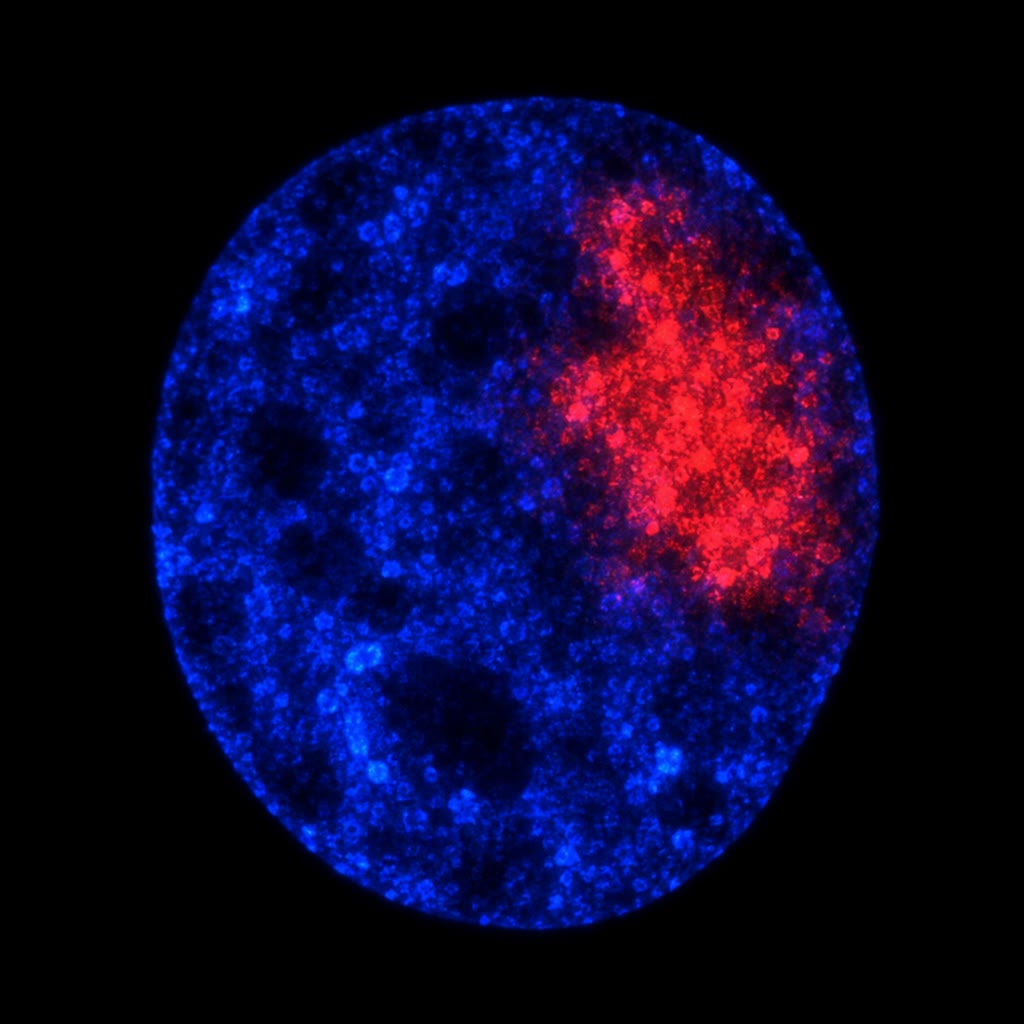
\includegraphics[width=0.36\linewidth]{images/book5/ai/b5-02-lncrna-nucleus.jpg}

{\small Un \omterm{def:b3:rna-regulation:ncrna}{ARN largo no codificante} en acción: el transcrito de
\emph{\omterm{def:b3:chromatin-epigenetics:x-inactivation}{Xist}} (rojo), detectado por hibridación fluorescente, recubre el
territorio de uno de los cromosomas X de un núcleo femenino (el ADN, en
azul).}
\end{omfigure}

\begin{remark}[Lo que aporta el control postranscripcional]\label{rem:b3:rna-regulation:why}
El control transcripcional actúa a través del núcleo, con un retraso de
minutos a horas antes de que un mensajero nuevo se fabrique, se exporte y
se traduzca. El control sobre el propio mensajero actúa donde la proteína
hace falta, en segundos o minutos, y puede ser local: una sola dendrita
que traduce un mensajero en una sinapsis, el borde delantero de un
fibroblasto que fabrica actina allí donde repta. Además convierte un gen
en muchas proteínas y permite que una sola señal --- el hierro, un
aminoácido, un \omterm{def:b3:rna-regulation:ncrna}{microARN} --- coordine centenares de mensajeros a la vez
sin tocar un solo promotor.
\end{remark}

\section{Ejercicios}

\begin{exercise}[$\star$]\label{exo:b3:rna-regulation:1}
Distínganse miARN, \omterm{def:b3:rna-regulation:ncrna}{ARNip} y \omterm{def:b3:rna-regulation:ncrna}{ARNpi} por su origen, su longitud, su
dependencia de \omterm{def:b3:rna-regulation:rnai}{Dicer} y lo que hacen a sus dianas.
\end{exercise}

\begin{exercise}[$\star$]\label{exo:b3:rna-regulation:2}
Sígase la biogénesis de un \omterm{def:b3:rna-regulation:ncrna}{microARN} desde su gen hasta un mensajero
reprimido, nombrando la enzima de cada corte.
\end{exercise}

\begin{exercise}[$\star$]\label{exo:b3:rna-regulation:3}
¿Por qué la inyección de ARN con sentido de \emph{unc-22} en gusanos
silenciaba el gen en los primeros experimentos, y qué cambiaron Fire y
Mello?
\end{exercise}

\begin{exercise}[$\star$]\label{exo:b3:rna-regulation:4}
¿Qué les ocurre a la ferritina y al receptor de transferrina cuando una
célula pasa hambre de hierro? ¿Qué paso de la expresión se controla en
cada caso?
\end{exercise}

\begin{exercise}[$\star\star$]\label{exo:b3:rna-regulation:5}
Un mensajero tiene una semivida de \qty{2}{h} y se fabrica a $5$
moléculas por minuto. Calcúlense su nivel estacionario y, después, el
nivel y el semitiempo cuando un \omterm{def:b3:rna-regulation:ncrna}{microARN} duplica su velocidad de
degradación.
\end{exercise}

\begin{exercise}[$\star\star$]\label{exo:b3:rna-regulation:6}
Una semilla de siete nucleótidos coincide con una secuencia al azar con
probabilidad $4^{-7}$. En un conjunto de \num{20000} mensajeros con
regiones 3$'$ no traducidas de \qty{1000}{nt} de media, ¿con cuántos
sitios coincide por azar una semilla de \omterm{def:b3:rna-regulation:ncrna}{microARN}? ¿Qué distingue
entonces a una diana real?
\end{exercise}

\begin{exercise}[$\star\star$]\label{exo:b3:rna-regulation:7}
Predígase el sexo de una mosca (a) con una mutación de pérdida de función
de \emph{tra} y dos cromosomas X; (b) que expresa TRA desde un transgén
constitutivo, con un solo X; (c) que carece del todo de \emph{dsx}.
\end{exercise}

\begin{exercise}[$\star\star$]\label{exo:b3:rna-regulation:8}
El mensajero de un protooncogén tiene normalmente una semivida de
\qty{15}{min} por un \omterm{def:b3:rna-regulation:stability}{elemento rico en AU}. Una translocación cromosómica
elimina el elemento y la semivida pasa a \qty{3}{h}. ¿Por qué factor sube
el nivel de proteína, si la traducción y la degradación de la proteína no
cambian? ¿Por qué es esto oncogénico aunque la proteína sea normal?
\end{exercise}

\begin{exercise}[$\star\star$]\label{exo:b3:rna-regulation:9}
Una cepa de laboratorio de \emph{Drosophila} carece de elementos P; una
cepa silvestre los lleva. Predígase la fertilidad de la descendencia de
(a) hembras de laboratorio $\times$ machos silvestres, (b) hembras
silvestres $\times$ machos de laboratorio, y explíquese la asimetría con
los \omterm{def:b3:rna-regulation:ncrna}{ARNpi}.
\end{exercise}

\begin{exercise}[$\star\star\star$]\label{exo:b3:rna-regulation:10}
Usando el \cref{thm:b3:rna-regulation:mirna-kinetics}, arguméntese que la
proteína fabricada a partir de un mensajero fluctúa menos, en términos
relativos, cuando el mensajero está bajo control de un \omterm{def:b3:rna-regulation:ncrna}{microARN}, a igual
nivel medio de mensajero. (La proteína promedia el mensajero a lo largo
de su propia vida, y el mensajero se renueva más deprisa.) ¿Por qué
podría una célula pagar un \omterm{def:b3:rna-regulation:ncrna}{microARN} y una velocidad de transcripción
mayor para obtener la misma media?
\end{exercise}

\begin{exercise}[$\star\star\star$]\label{exo:b3:rna-regulation:11}
En los gusanos, una ARN-polimerasa dependiente de ARN fabrica \omterm{def:b3:rna-regulation:ncrna}{ARNip}
secundarios a partir del mensajero diana; en los mamíferos no hay
ninguna. Predígase, para cada uno, si el silenciamiento por una sola
inyección de ARN de doble hebra dura a lo largo de muchas divisiones
celulares y si se propaga a otros tejidos, y explíquese la consecuencia
médica para los fármacos de \omterm{def:b3:rna-regulation:ncrna}{ARNip}.
\end{exercise}

\begin{exercise}[$\star\star\star$]\label{exo:b3:rna-regulation:12}
Un lncARN recién anotado se expresa en el corazón. Diséñense los
experimentos que distinguirían (a) un ARN funcional, (b) un acto de
transcripción funcional cuyo ARN es irrelevante y (c) ruido, y dígase qué
resultado predice cada uno.
\end{exercise}

\section{Problema: el temporizador de un gusano}

\begin{problem}[{Problema de fin de semana --- el interruptor
\emph{lin-4}/\emph{lin-14} del gusano temporizado con la cinética del
mensajero, un ARN inyectado que se diluye a lo largo de las divisiones de
un embrión y al que rescata la amplificación, el regulón del hierro
cuantificado y un recuento de cortes y empalmes, hasta llegar al factor
de represión, al semitiempo del interruptor y al número de divisiones que
sobrevive una señal sin amplificar}]
\label{pb:b3:rna-regulation:1}
Datos: el mensajero de \emph{lin-14} se fabrica a $k = 3$ moléculas por
minuto y por célula y tiene una semivida de \qty{40}{min}. La proteína
LIN-14 se fabrica a $\beta = 2$ por mensajero y por minuto y tiene una
semivida de \qty{3}{h}. Desde el comienzo del segundo estadio larvario,
el ARN de \emph{lin-4} se acumula y añade un término de degradación
$\gamma' R = 3\gamma$ al mensajero y, al bloquear la iniciación, reduce
$\beta$ a la mitad. Un embrión de gusano pasa de una célula a unas
\num{550} al eclosionar; un adulto tiene \num{959} células somáticas.

\medskip
\noindent\textbf{Parte I --- El mensajero.}
\begin{enumerate}
  \item Calcúlense $\gamma$ y el nivel estacionario del mensajero de
        \emph{lin-14} antes de que aparezca \emph{lin-4}.
  \item Calcúlense la velocidad de degradación de la proteína y el nivel
        estacionario de la proteína LIN-14.
  \item Una vez presente \emph{lin-4}, calcúlense el nuevo nivel del
        mensajero y su nueva constante de tiempo.
  \item Calcúlense el nuevo estado estacionario de la proteína y el
        factor global de represión sobre la proteína.
  \item ¿Cuánto tarda el mensajero, desde que aparece \emph{lin-4}, en
        recorrer la mitad del camino hasta su nuevo nivel? ¿Y la
        proteína? ¿Qué paso limita la velocidad del interruptor?
  \item Los experimentos originales encontraron la proteína ausente
        mientras el ARNm seguía siendo detectable. ¿Es esto coherente
        con los números obtenidos? ¿Qué fracción del mensajero queda?
\end{enumerate}

\medskip
\noindent\textbf{Parte II --- Dilución y amplificación.}
\begin{enumerate}[resume]
  \item Se inyectan en la gónada de un gusano $10^{6}$ moléculas de ARN
        de doble hebra, que se reparten por igual entre \num{250}
        huevos. ¿Cuántas moléculas por huevo?
  \item Si las moléculas se repartieran sin más en cada división,
        ¿cuántas tendría cada célula de la larva de \num{550} células al
        eclosionar? ¿Tras cuántas divisiones más bajaría la media de una
        por célula?
  \item Fire y Mello vieron el silenciamiento en todo el animal y en su
        descendencia, a unas pocas moléculas por célula. Explíquese qué
        añade una ARN-polimerasa dependiente de ARN a esta explicación, y
        por qué el efecto se desvanece de todos modos al cabo de unas
        pocas generaciones.
  \item En una célula de mamífero sin esa polimerasa, una transfección
        de \omterm{def:b3:rna-regulation:ncrna}{ARNip} mete \num{5000} dúplex en una célula que se divide a
        diario; el \omterm{def:b3:rna-regulation:rnai}{RISC} es estable pero la división lo diluye. ¿Tras
        cuántos días baja el recuento de \num{100}, aproximadamente el
        número necesario para un silenciamiento eficaz?
  \item Un \omterm{def:b3:rna-regulation:ncrna}{ARNip} terapéutico contra un mensajero hepático se administra
        una sola vez y funciona seis meses. Los hepatocitos apenas se
        dividen. Explíquese por qué el mecanismo de la pregunta 10 no lo
        limita, y qué sí lo limita.
  \item Una semilla de siete nucleótidos coincide al azar una vez cada
        $4^{7}$ nucleótidos. El transcriptoma del gusano tiene unas
        \qty{20}{Mb} de secuencia 3$'$ no traducida. ¿Cuántas
        coincidencias de semilla por azar tiene \emph{lin-4}, y cómo
        supieron los genetistas qué diana importaba?
\end{enumerate}

\medskip
\noindent\textbf{Parte III --- El regulón del hierro.}
\begin{enumerate}[resume]
  \item En células ricas en hierro el mensajero del receptor de
        transferrina tiene una semivida de \qty{10}{min}; con la IRP
        unida, de \qty{50}{min}. Sin cambios en la transcripción, ¿por
        qué factor sube el mensajero cuando el hierro escasea?
  \item El mensajero de la ferritina no cambia de nivel, pero su
        traducción baja de $1$ a $0.05$ proteínas por mensajero y por
        minuto cuando se une la IRP. ¿Por qué factor cae la síntesis de
        ferritina?
  \item Combínense ambos: ¿por qué factor cambia la razón entre la
        capacidad de importación y la de almacenamiento entre los
        estados rico y pobre en hierro?
  \item La proteína IRP1 es o bien una proteína de unión al ARN o bien
        una aconitasa, según lleve o no un agregado de hierro y azufre.
        Explíquese por qué esto la convierte en un sensor del propio
        hierro y no de una hormona.
  \item Un paciente lleva una mutación del IRE de la ferritina que
        anula la unión de la IRP. Predíganse el nivel de ferritina, el
        hierro sérico y por qué se afecta el cristalino del ojo.
  \item Explíquese en una frase por qué la misma horquilla puede activar
        en una posición y reprimir en otra.
  \item La IRP2 no tiene agregado de hierro y azufre; cuando el hierro
        abunda la destruye una ubiquitina-ligasa cuya propia estabilidad
        exige hierro y oxígeno. ¿Por qué podría una célula mantener dos
        sensores de química tan distinta?
\end{enumerate}

\medskip
\noindent\textbf{Parte IV --- Contar isoformas.}
\begin{enumerate}[resume]
  \item \emph{Dscam} tiene bloques de exones con 12, 48, 33 y 2
        alternativas mutuamente excluyentes. ¿Cuántas isoformas? Si cada
        neurona expresa unas $50$ al azar, ¿cuál es la probabilidad de
        que dos neuronas dadas compartan al menos una? (Úsese $1 - (1 -
        50/N)^{50}$.)
  \item ¿Por qué le conviene a una neurona tener isoformas que sus
        vecinas casi con seguridad no tienen?
  \item Un gen con $n$ exones de casete, cada uno incluido o saltado de
        forma independiente, ¿cuántos mensajeros da? ¿Cuántos para
        $n = 10$? ¿Por qué el número real en un tipo celular dado suele
        ser mucho menor?
  \item En la mosca, ¿por qué una hembra con dos cromosomas X pero un
        alelo nulo de \emph{Sxl} muere en lugar de desarrollarse sin más
        como macho? (Considérese qué más controla el sistema de recuento
        de X: la \omterm{def:b3:chromatin-epigenetics:x-inactivation}{compensación de dosis} de los genes ligados al X.)
  \item SXL favorece el corte y empalme productivo de su propio
        transcrito. Explíquese por qué esto convierte la decisión sexual
        en una memoria que persiste después de que haya desaparecido la
        señal de recuento de X, presente solo en el embrión temprano, y
        relaciónese con los interruptores autosostenidos del
        \cref{ch:b3:chromatin-epigenetics}.
  \item Resúmase el temporizador: el factor de represión sobre la
        proteína LIN-14 (pregunta~4), el semitiempo del interruptor del
        mensajero (pregunta~5) y el número de divisiones que sobrevive
        una señal sin amplificar antes de caer por debajo de una
        molécula por célula (pregunta~8).
\end{enumerate}
\end{problem}
